\section{Visualization of TensorFlow Graphs}\label{sec:visual}

Deep-learning models often employ very wide and especially very deep neural
networks, composed of computational graphs with a highly complex and intricate
structure. For example, \cite{inception} reports of deep convolutional network
based on the Google \emph{Inception} model with more than 36,000 individual
units, while \cite{tensorflow} states that certain long short-term memory (LSTM)
architectures can span over 15,000 nodes. To maintain a clear overview of such
complex networks and be able to observe and inspect changes on various levels in
detail, powerful visualization tools are required. \emph{TensorBoard}, a
web-interface for TensorFlow graph visualization and manipulation, is an example
for such a tool. It is built directly into the TensorFlow library and thus
integrates well. In this section, we first list a number of noteworthy features
of TensorBoard and then discuss how it may be used from TensorFlow's programming
interface.

\subsection{TensorBoard Features}\label{sec:visual-features}

The core feature of TensorBoard is the lucid visualization of computational
graphs, exemplified in Figure \ref{fig:tensorboard-a}. Graphs with complex
topologies and many layers can be displayed in a clear and organized manner,
allowing the user to understand exactly how data flows through it. Especially
useful is TensorBoard's notion of \emph{name scopes}, whereby nodes or entire
subgraphs may be grouped into one visual block, such as a single neural-network
layer. Such name scopes can then be expanded interactively to show the grouped
units in more detail. Figure \ref{fig:tensorboard-b} shows the expansion of one
the name scopes of Figure \ref{fig:tensorboard-a}.

Furthermore, TensorBoard allows the user to track the development of individual
tensor values over time. For this, you can attach two kinds of \emph{summary
  operations} to nodes of the computational graph: \emph{scalar summaries} and
\emph{histogram summaries}. Scalar summaries show the progression of a scalar
tensor value, which can be sampled at certain iteration-counts. In this way, you
could, for example, observe the accuracy or loss of your model with
time. Histogram summary nodes allow the user to track value
\emph{distributions}, such as those of neural-network weights or the final
softmax estimates. Figures \ref{fig:tensorboard-c} and \ref{fig:tensorboard-d}
give examples of scalar and histogram summaries, respectively. Lastly,
TensorBoard also allows visualization of images. This can be useful to show the
images sampled for each mini-batch of an image classification task, or to
visualize the kernel filters of a convolutional neural network
\cite{tensorflow}.

We note especially how interactive the TensorBoard web-interface is. Once your
comptutational graph is uploaded, you can pan and zoom the model as well as
expand or contract individual name scopes. A demonstration of TensorBoard is
available at \emph{https://www.tensorflow.org/tensorboard/index.html}.

\subsection{TensorBoard in Practice}\label{sec:visual-code}

To integrate TensorBoard into your TensorFlow code, three steps are
required. Firstly, it is wise to group nodes into \emph{name scopes}, as
discussed above. Then, you may add scalar and histogram summaries to you
operations. Finally, you must instantiate a \texttt{SummaryWriter} object and
hand it the tensors produced by the summary nodes in a session context whenever
you wish to store new summaries. Rather than fetching individual summaries, it
is also possible to combine all summary nodes into one via the
\texttt{tf.merge\_all\_summaries()} operation.

\lstinputlisting{code/visual.py}

\begin{figure}[h!]
  \centering
  \begin{subfigure}[h]{0.5\textwidth}
    \centering
    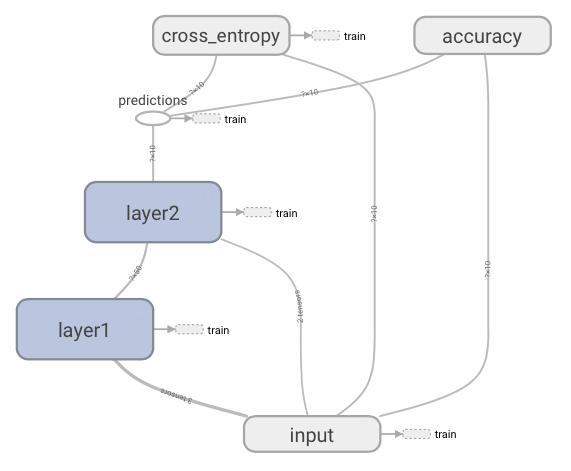
\includegraphics[scale=0.4]{no-train}
   \caption{}
   \label{fig:tensorboard-a}
  \end{subfigure}

  \vspace{0.3cm}

  \begin{subfigure}[h]{0.5\textwidth}
    \centering
    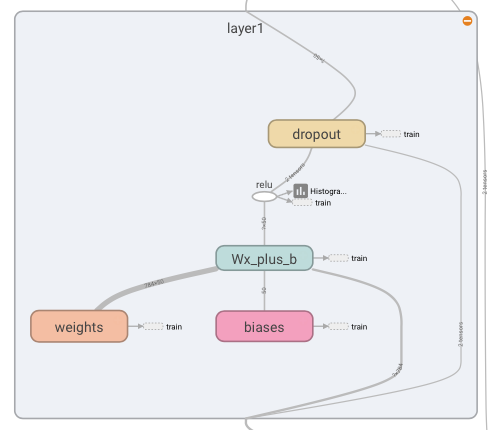
\includegraphics[scale=0.4]{layer1}
    \caption{}
    \label{fig:tensorboard-b}
  \end{subfigure}

  \vspace{0.3cm}

  \begin{subfigure}[h]{0.2\textwidth}
    \centering
    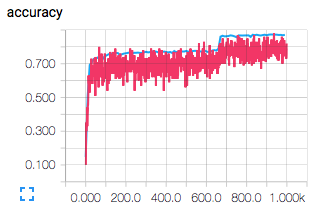
\includegraphics[scale=0.35]{accuracy}
    \caption{}
    \label{fig:tensorboard-c}
  \end{subfigure}
  %
  \begin{subfigure}[h]{0.2\textwidth}
    \centering
    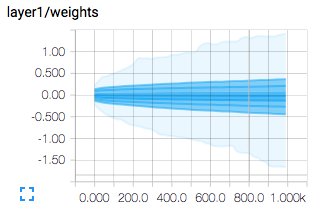
\includegraphics[scale=0.35]{blue-weights}
    \caption{}
    \label{fig:tensorboard-d}
  \end{subfigure}
  \caption{Foo}
  \label{fig:tensorboard}
\end{figure}

%%% Local Variables:
%%% mode: latex
%%% TeX-master: "../paper"
%%% End: